\documentclass{article}
\usepackage{graphicx} % Required for inserting images
\usepackage{float}
\usepackage{adjustbox}



\title{KTH DD2391 - Project report\\[0.3cm]
\scshape{actionlens - A Security Analysis of GitHub Actions Workflows}}
\author{\underline{Group 14:} \\[0.3cm]
Alexander Götting, Chinmay Prawah Pant, \\
Elsa Kieffer, Tilda L. Aderud}
\date{\today}

\begin{document}

\maketitle

\section{Introduction}

Continuous Integration and Continuous Deployment (CI/CD) is a large part of modern day software development and is used for automating processes, such as testing or building \cite{githubcicd}. GitHub Actions is one of the most commonly used CI/CD forums. This is because they allow their users to define their own automated workflows (also called Actions) using easily-read configuration files (YAML-files) \cite{githubactions}. But, with this automation also comes security issues. Since the workflows can execute code, access repository information, use authentication tokens and secrets, as well as invoke third-party Actions, a vulnerable or over privileged workflow can have serious consequences. A successful exploitation might expose these authentication tokens/secrets or accidentally modify repositories \cite{koishybayev2022}. One can only imagine how much worse it could get if a person with bad intentions manages to get control of one of those files.

Previous research in this field shows that 99.8\% of GitHub Actions workflows are over-privileged or have some sort of related security concern. Recent work, such as \textsc{Argus}, analyzed almost 2.8 million workflows and saw thousands of code-injection vulnerabilities \cite{muralee2023}.

Our goal of this project is to investigate if a security-focused static analyzer more easily can identify a limited set of unsafe GitHub Actions patterns. Actionlens uses a combination of structural linting and semantic data-flow analysis. This is therefore not a general analysis framework, but rather focuses on a predefined set of GitHub Actions vulnerabilities.

The analyzer starts by parsing and inspecting GitHub Actions YAML files into a normalized representation by using the \texttt{actionlint} parser \cite{actionlint}. Relevant workflow information is converted into a Abstract Syntax Tree (AST) and passed to the Python analysis engine. Next, the static analyzer applies two techniques: Linting that performs structural and configuration checks whilst the semantic analysis part tracks potentially untrusted data via sources to (security-sensitive) sinks. The findings are finally presented through a command line report or alternatively as a JSON output. 

\section{Background}

\subsection{Github Actions workflows}

Normally, GitHub Actions workflows are YAML files that is stored under the \texttt{.github/workflows/} path. A workflow specifies event(s) that trigger an execution, such as \texttt{push}, \texttt{pull\_request} or \texttt{pull\_request\_target}. It then defines one or several jobs, where each job explain a sequence of individual steps \cite{githubactions}. An example is the following YAML-file: 

\begin{verbatim}
(1)    on: 
(2)        pull_request:
(3)
(4)    jobs:
(5)        test:
(6)            runs-on: ubuntu-latest
(7)            steps:
(8)                - uses: actions/checkout@v4
(9)                - run: make test
\end{verbatim} 

\textit{This is an example of a workflow that is triggered when a pull request} \texttt{(2)} \textit{is opened/updated. It contains a job named} \texttt{test (5)} \textit{which runs on an Ubuntu runner} \texttt{(6)}\textit{, and the job consists of two steps. First step:} \texttt{actions/checkout@v4 (8)}\textit{, is used to check out the repository content onto the runner. The second step is}  \texttt{make test (9)}\textit{, which is executed in a shell. What this means is that the workflow automatically gets the repository code and runs the projects test procedure when a pull request is triggered \cite{githubactions}.} \\

Individual steps may for example execute shell commands, invoke external Actions, interact with APIs or use secrets/token. Workflow authors should therefore consider the origin of input values as well as the trustworthiness of third party Actions and permissions of automatically generated \texttt{GITHUB\_TOKEN}s \cite{githubsecurity}. Additionally, it is important to consider whether or not an attacker controlled pull-request may be able to reach privileged execution contexts \cite{githubprtarget}. 

\subsection{Static security analysis}

In general terms, a static analysis examines a program without actually running the code \cite{ibmstatic}. In this project, the static analysis consists of two parts. 

The first part uses linting, where the parsed workflow structure is inspected for any relevant patterns regarding configuration security issues, such as unpinned third-party Actions. These rules primarily run on the normalized workflow AST. 

The second part is a semantic and taint-based data flow analysis. Here, potential attacker-controlled values will be tracked from their source, through intermediate workflow constructs to security sensitive sinks. Security problems in this area usually refers to how data actually is used, rather than only on the presence of security sensitive patterns. An example of this is an attacker-controlled GitHub context expression that is interpolated directly to a shell command. 

\section{Threat Model}

\subsection{Assets}

The main assets we consider are the repository contents, authentication tokens, repository secrets, the workflow execution environment, and the CI/CD process itself.

GitHub Actions workflows can access repository contents and are given a
\texttt{GITHUB\_TOKEN} when they run. Depending on its permissions, this token can be used to read or modify parts of the repository. Workflows can also have access to repository secrets, such as API keys or other credentials \cite{githubtoken,githubsecurity}. If a workflow is vulnerable, these resources could potentially be exposed or misused by an attacker \cite{githubrunners}.

Another important asset is the workflow execution environment. Since GitHub Actions can execute commands on runners, an attacker who manages to influence these commands could also affect the environment in which the workflow runs \cite{githubrunners}. Finally, we consider the integrity of the CI/CD process itself an asset. The workflow should perform the tasks intended by the repository owner without allowing external input to change its behaviour in an unsafe way.


\subsection{Attacker Model}

We mainly consider an external GitHub user who does not have write or administrative access to the target repository. However, an external user may still be able to interact with the repository, for example by opening a pull request, creating an issue, or writing a comment.

Some information controlled by these users can be accessed by workflows through the \texttt{github} context. This includes, for example, pull request titles and bodies, issue titles, comments, and some branch-related values \cite{githubcontexts,githubscriptinjection}. This means that an attacker can potentially provide input to a workflow without being able to modify the workflow file itself \cite{githubscriptinjection}.

In our threat model, we therefore assume that the attacker tries to influence the workflow through these external inputs. The attacker is not assumed to already have administrative control of the repository. A security problem can occur when attacker-controlled data is used in a sensitive operation, such as a shell command, especially if the workflow also has access to sensitive repository resources \cite{githubscriptinjection,githubsecurity}.

\subsection{Threats Considered}

The threats considered in this project correspond to the six security problems that ActionLens aims to detect: script injection, excessive \texttt{GITHUB\_TOKEN} permissions, unpinned third-party Actions, untrusted Action namespaces, unsafe use of self-hosted runners, and unsafe use of privileged pull-request workflows. 

Script injection may occur when attacker-controlled input is used directly in a shell command. In such a case, an attacker may be able to change the command that is executed by the workflow rather than only providing data to it \cite{githubscriptinjection}. % Do we want to mention that we divide the rules into two categories: Linting and Code-analysis ?

Excessive \texttt{GITHUB\_TOKEN} permissions are considered a threat because a workflow may be given more access to repository resources than it actually needs. This does not necessarily represent a vulnerability on its own, but it can increase the impact of another vulnerability if the workflow becomes compromised \cite{githubtoken,githubsecurity}.

Third-party Actions are considered a potential threat when they are not pinned to an immutable version. If the referenced Action changes, the code executed by the workflow may also change without any modification to the workflow itself \cite{githubsecurity,owaspactions}.

Action namespaces are also considered because a workflow may reference an
Action from an unexpected or potentially untrusted owner. This includes cases
such as names that are similar to trusted namespaces or known Action repository
names appearing under an unexpected owner. Such references may indicate
typosquatting or the use of an unintended third-party Action.

Self-hosted runners are considered a threat because workflow jobs execute on
infrastructure controlled by the repository owner or organization. The risk is
particularly relevant when a self-hosted runner is used together with triggers
that can be influenced by external users, such as pull requests or issue
comments. In such cases, untrusted input may affect workflow execution on
persistent infrastructure.

Finally, privileged pull-request workflows are considered because they may combine input originating from an untrusted pull request with access to sensitive repository resources. This becomes particularly security-relevant when attacker-controlled data or code can influence a workflow running in a privileged context \cite{githubprtarget,owaspactions}.

\subsection{Scope and Assumptions}

Our threat model focuses on security problems that can be identified from the structure and data available in GitHub Actions workflow files. We assume that the workflow file itself was created by a trusted repository maintainer, while some of the data processed by the workflow may originate from untrusted external users.

The attacker is not assumed to already have write or administrative access to the repository. An attacker with such privileges could directly modify repository contents or workflows, which is outside the attacker model considered in this project. We instead focus on cases where a less privileged user can influence workflow execution through normal GitHub interactions, such as pull requests, issues, comments, or related metadata.

ActionLens is intentionally limited to a predefined set of GitHub Actions security patterns and is not intended to provide a complete security analysis of a repository. Vulnerabilities in GitHub itself, compromised maintainer accounts, and general vulnerabilities in the application source code are outside the scope of the project. The analysis is therefore limited to the GitHub Actions related threats explicitly considered by ActionLens.

\section{Related Work}

\subsection{\textsc{\textmd{Argus}}}

\textsc{Argus} is a static taint framework for GitHub workflows and Actions. Instead of only using basic patterns (also known as linting) to sense vulnerabilities it models the flow of attacker-controlled data from sources to security-sensitive sinks \cite{muralee2023}. 

When the authors compared their framework to already existing linting based scanners \textsc{Argus} seemed to have 7 times higher vulnerability discovery rate \cite{muralee2023}. 

The scope of \textsc{Argus} is substantially more complex than our limited project, but will still be relevant because of its expression injection component. The difference in the two projects is the sheer volume. Whilst \textsc{Argus} is a finalized and ready-to-use analyzer, our project aims to investigate what can be achieved when a smaller and more explainable security rule set is used. \textsc{Argus} is also extremely relevant to our project since both systems reason about attacker-controlled data which flows from sources to sinks. Since our project also implements a small taint-analysis model, \textsc{Argus} serves as both related work and a good reference point when designing our semantic analysis component.

\subsection{GitHub's CodeQL}

The GitHub CodeQL is made to query GitHub Actions workflow files, specifically checking for security issues regarding configurations/expressions \cite{githubcodeql}. GitHub Security Lab has already reported that they have started using CodeQL to identify vulnerability patterns such as unnecessary use of \texttt{pull\_request\_target} \cite{githubsecuritylabcodeql}. 

Differently to our project, CodeQL is a general analysis framework with a huge query system \cite{githubcodeql}. 

\subsection{zizmor}

zizmor is a static open-source analysis tool for CI/CD setups. It supports several automated configuration formats, and among those are GitHub Actions. The tool checks for template injection, credential exposure, excessive permissions and unsafe Git references, but also supports several other automated security workflow concepts \cite{zizmor}. 

\subsection{OpenSSF Scorecard}

OpenSSF Scorecard looks at open-source repositories for security issues \cite{scorecard}. For example, it may identify known dangerous GitHub Actions patterns such as script injection or non-trusted code checkouts. The untrusted checkout analysis tool specifically searches for workflows triggered by \texttt{pull\_request\_target} or \texttt{workflow\_run} which explicitly looks at pull request controlled references \cite{scorecard}. 

Similarly to our project, OpenSSF Scorecard is purely static, meaning that it does not check whether the potentially dangerous pattern it identified actually might be handled in a safely manner. However, Scorecard evaluates a broader set of security practices at repository-level, whilst Actionlens focuses on workflow structure and data-flow vulnerabilities.

\subsection{Checkov}

Checkov is a broad security and policy-as-code (rules/constraints) scanner \cite{checkov,ibmpolicy}. It also supports GitHub Actions as well as CI/CD configuration files, which includes graph-based policies and being able to make custom checks \cite{checkov}. 

The scope of Checkov is much broader than the scope of our project since Checkov also support several configuration formats such as YAML and JSON to only name a few. Checkov is a good example of how security rules can be represented, reported and integrated \cite{checkov}. 

\subsection{actionlint}

Like many of the other similar related work, actionlint is a static checker for GitHub Actions. It checks several different correctness/security oriented problems such as YAML syntax, GitHub expression types, hard-coded credentials and reusable workflows \cite{actionlint}. 

The tool is mainly used for detecting mistakes and linting rather than noticing major security errors and deciding their consequences \cite{actionlint}. 

Actionlens uses actionlint as the parsing frontend rather than implementing any GitHub Actions parser from scratch. The workflow is then converted into a normalized AST and analyzed in Actionlens using security rules. actionlint is therefore both related and directly implemented which makes it a dependency in our project. The security analysis logic of Actionlens is implemented separately though. 

\section{Design and Implementation}

ActionLens is implemented as a static analysis pipeline for GitHub Actions workflow files. The system separatesworkflow parsing from the security
analysis The complete analysis process can be divided into several stages, starting with a YAML workflow file and ending with a set of security findings. A Go frontend based on \texttt{actionlint} parses the workflow
and produces a normalized representation, which is then analyzed by the
Python security engine. 

This creates the following overall architecture:

\begin{verbatim}
       GitHub Actions Workflow (YAML)
                   |
          Go / actionlint Parser
                   |
          Normalized AST / JSON
                   |
          Python Analysis Engine
                   |
          +--------+--------+
          |                 |
   Linting Rules   Taint Analysis (NetworkX)
          |                 |
          +--------+--------+
                   |
            Security Findings
                   |
          +--------+--------+
          |                 |
     Terminal Output    JSON Output
\end{verbatim}

\subsection{Workflow Parsing and Internal Representation}

GitHub Actions workflows are written in YAML, but simply treating them as regular YAML files would not give enough information for the security analysis in ActionLens. A workflow also contains GitHub Actions-specific concepts, such as triggers, jobs, steps, runner configurations, permissions, \texttt{run} commands, \texttt{uses} statements, and expressions written as \texttt{\$\{\{ ... \}\}}. Because of this, ActionLens uses a parser that can understand the specific structure of GitHub Actions workflows.

Actionlens does not implement a GitHub Actions parser from scratch, instead a Go frontend uses the \texttt{actionlint} library. The YAML workflow is first parsed using \texttt{actionlint}. The result is then converted into our own normalized Abstract Syntax Tree (AST). The main reason for doing this is to create a smaller and more consistent representation that only contains the information needed for the security analysis.

At the workflow level, the AST contains information about the workflow name, triggers, permissions, environment variables, jobs, and source positions. For triggers, information such as the event type can be stored together with filters for activity types, branches, tags, and paths. Permissions can either be represented as broader settings, such as \texttt{read-all} and \texttt{write-all}, or as separate permission scopes.

For each job, the parser extracts its identifier and name, runner configuration, permissions, dependencies defined with \texttt{needs}, conditional expressions, environment variables, outputs, and steps. The runner configuration also contains information about runner labels and groups when these are specified in the workflow.

The steps are represented in a similar way. Information such as the step identifier, name, condition, execution type, environment variables, and source position is stored. For shell execution steps, the AST contains the \texttt{run} command and shell configuration. For steps using an Action, the \texttt{uses} reference is separated into the owner, repository, and reference. The parser also checks whether the reference follows the expected 40-character commit SHA format. However, it does not verify that the SHA corresponds to an existing Git commit. This information can later be used by rules that check how third-party Actions are referenced.

GitHub expressions are extracted from the relevant fields of a step. Currently, the parser looks for expressions inside \texttt{run}, \texttt{if}, \texttt{env}, and \texttt{with}. The expression itself is then parsed using the expression parser from \texttt{actionlint}. For example, an expression such as \texttt{github.event.issue.body} can be stored together with information about where it appeared, for example inside a \texttt{run} command or an environment variable. This becomes important for the code and taint analysis, where we need to identify how potentially untrusted values are used in a workflow.

The parser also keeps source positions for several parts of the workflow, including jobs, steps, runner configurations, and permissions. These contain the line and column in the original workflow file and can therefore be used to connect a security finding to its location in the file.

When the Go parser has created the normalized AST, it is serialized into JSON and passed to the Python part of ActionLens. The Python component runs the Go parser as a separate process and reads the resulting JSON. Pydantic models are then used to validate the data and convert it into a Python \texttt{WorkflowAST}. These models represent the same main structures as the Go parser, including workflows, jobs, steps, triggers, permissions, runner configurations, Action references, expressions, and source positions.

With this structure, the security rules do not have to parse the original YAML themselves. Both the linting rules and the code-analysis rules can instead work with the same \texttt{WorkflowAST}. It also keeps the GitHub Actions-specific parsing separate from the security analysis implemented in Python.

\subsection{Security Analysis}

After the workflow has been parsed, the normalized AST is passed to the Python analysis engine. ActionLens uses a predefined set of security rules, where each rule looks for a specific type of insecure configuration or behavior in the workflow. The goal is not to detect every possible GitHub Actions vulnerability, but to focus on the security issues included in the scope of the project.

The static analysis is divided into two main parts: security linting and code analysis. The \texttt{AL-LINT} rules mainly analyze the structure and configuration of the workflow AST. These rules inspect properties such as action references, permissions, and runner configurations without constructing a data-flow graph. The \texttt{AL-CODE} rules are used for vulnerabilities that require more information about how different parts of the workflow interact. These rules include taint analysis, where potentially untrusted inputs are tracked to determine whether they can reach security-sensitive operations, such as shell commands in a \texttt{run} step.

When a rule detects a security issue, it produces a finding. The findings use a common format containing the rule identifier, severity, workflow file, source line, a description of the issue, and a suggested remediation. Using the same format makes it possible to report findings in the same way regardless of which security rule produced them.

The security rules included in ActionLens are summarized in Table~\ref{tab:security-rules}.

\begin{table}[h]
    \centering
    \caption{Security rules included in ActionLens.}
    \begin{adjustbox}{width=1.4\textwidth, center=\textwidth}
        \begin{tabular}{lllll}
        \hline
        \textbf{Rule} & \textbf{Type} & \textbf{Description} & \textbf{OWASP CI/CD Mapping} & \textbf{CWE} \\
        \hline
        AL-LINT-001 & Lint & Unpinned third-party action & CICD-SEC-4: \textit{Poisoned Pipeline Execution} & CWE-94 \\
        AL-LINT-002 & Lint & Untrusted action namespace & CICD-SEC-4: \textit{Poisoned Pipeline Execution} & CWE-829 \\
        AL-LINT-003 & Lint & Missing or over-scoped permissions & CICD-SEC-3: \textit{Dependency Chain Abuse} & CWE-494 \\
        AL-LINT-004 & Lint & Unsafe self-hosted runner usage & CICD-SEC-3: \textit{Dependency Chain Abuse} & CWE-829 \\
        AL-CODE-001 & Code & Script injection & CICD-SEC-5: \textit{Insufficient PBAC} & CWE-250 \\
        AL-CODE-002 & Code & Untrusted checkout on privileged trigger & CICD-SEC-7: \textit{Insecure System Configuration} & CWE-668 \\
        \hline
    \end{tabular}
    \end{adjustbox}
    \label{tab:security-rules}
\end{table}

\subsubsection{Security Linting}

The security linting part of ActionLens looks for insecure configurations and structural patterns in the workflow AST. Unlike the taint analysis, these rules do not need to construct a data-flow graph between a source and a sink. Instead, they inspect information that has already been extracted by the parser, such as \texttt{uses} references, permissions, runner configurations, and workflow triggers.

The first rule, \texttt{AL-LINT-001}, detects unpinned third-party Actions. When an Action is referenced through a \texttt{uses} statement, the rule checks whether the reference follows the expected format of a full 40-character commit SHA. References to mutable tags or branches, such as \texttt{actions/checkout@v4}, are reported because the code associated with these references may change over time. ActionLens only checks the format of the reference and does not verify that the SHA corresponds to an existing Git commit.

\texttt{AL-LINT-002} focuses on potentially untrusted Action namespaces. The rule can detect names that are similar to trusted namespaces, which may indicate typo-squatting. It also checks for known official Action repository names used under an unexpected owner. For example, an Action that uses the repository name \texttt{checkout} but is not owned by a trusted namespace can be considered suspicious. The rule also supports a stricter allowlist mode where Actions outside the configured trusted namespaces can be reported.

The third rule, \texttt{AL-LINT-003}, analyzes the permissions given to the
workflow's \texttt{GITHUB\_TOKEN}. The rule checks whether a top-level
\texttt{permissions} block is missing and detects broad
\texttt{write-all} permissions at both workflow and job level. The purpose is
to identify workflows where the token may have broader permissions than
necessary.

Finally, \texttt{AL-LINT-004} checks the use of self-hosted runners. If a job uses a runner with the \texttt{self-hosted} label together with an external or untrusted trigger, such as \texttt{pull\_request} or \texttt{issue\_comment}, the rule reports a high-severity finding. For internal triggers, such as \texttt{push} or \texttt{workflow\_dispatch}, the use of a self-hosted runner is instead reported as a medium-severity warning. This distinction is made because executing externally influenced workflows on persistent infrastructure can create a larger security risk.

\subsubsection{Code and Taint Analysis}

Some security problems cannot be identified only by looking for a specific configuration or keyword in the workflow. For example, the presence of a \texttt{run:} step is not itself a vulnerability. The security problem depends on what data reaches the command and where that data originates. ActionLens therefore uses taint analysis for vulnerabilities where attacker-controlled data may reach a security-sensitive operation.

The analysis follows a simplified source-to-sink model:
\begin{verbatim}
Source -> Propagator(s) -> Sink
\end{verbatim}

A source is a GitHub context value that may be controlled by an
external user. Examples include issue and pull-request titles or bodies,
comments, and branch-related values such as \texttt{github.head\_ref}. A
propagator represents how such a value is transferred through the
workflow, while a sink is a security-sensitive operation where the
value may become executable, especially a \texttt{run:} shell command.

ActionLens represents these relationships using a directed NetworkX graph.
Nodes represent relevant values or operations and edges represent possible
data flows. A path from an untrusted source to a security-sensitive sink can
therefore indicate a vulnerability.

The \texttt{AL-CODE-001} rule detects potentially untrusted GitHub context
expressions that are interpolated directly into a shell command. For example:
\begin{verbatim}
- run: echo "${{ github.event.comment.body }}"
\end{verbatim}

Since the comment body can be controlled by an external user, inserting it directly into the command may allow the input to affect the executed shell command. A safer pattern is to pass the expression through an environment variable:
\begin{verbatim}
- env:
    COMMENT_BODY: ${{ github.event.comment.body }}
  run: echo "$COMMENT_BODY"
\end{verbatim}

This separates the GitHub expression from direct interpolation into the shell script. 

The \texttt{AL-CODE-002} rule considers workflows triggered by
\texttt{pull\_request\_target}. Such workflows execute in the context of the base repository and can become dangerous if they explicitly check out attacker-controlled pull-request code. ActionLens therefore checks the relationship between the privileged trigger and the reference used by the checkout step. This is treated as environmental taint, where untrusted code is introduced into a more privileged execution context.

\subsection{Reporting and Command-Line Interface}

ActionLens provides a command-line interface for running the analysis on GitHub Actions workflow files. After the selected security rules have been executed, the resulting findings are collected and presented to the user.

Each finding contains information such as the rule identifier, severity,
workflow file and line number, together with a description of the detected
problem and suggested remediation.

The current implementation provides two output formats. The default output is
a human-readable terminal report, where findings are presented in a table. This makes it possible to quickly see which rule produced the finding, its
severity, where in the workflow it occurred, and how the problem can be
addressed.

ActionLens can also produce JSON output. In this format, the same findings are represented as structured data instead of a terminal table. This makes the results easier to process using other tools or scripts.

An example of the information contained in a finding is shown below: 
\begin{verbatim}
Rule:        AL-CODE-001
Severity:    HIGH
Location:    .github/workflows/example.yml:13
Message:     Untrusted expression interpolated
             directly into shell script sink.
Remediation: Pass the context value through an
             environment variable.
\end{verbatim}

SARIF output was considered during the design of ActionLens, but is not included in the final implementation.

\subsection{Implementation Decisions and Trade-offs}

Instead of building a complete GitHub Actions parser from scratch, we decided to build the parsing component around the existing \texttt{actionlint} library. Since \texttt{actionlint} already understands the structure of GitHub Actions workflows and their expressions, this reduced the amount of parsing logic that we had to implement ourselves. We then added our own processing around the library to create the normalized representation that is used by the rest of ActionLens.

The security analysis was implemented in Python. A practical reason for this was that we had more previous experience with Python than with Go, which made it easier to develop and test the different security rules. It also gave us a clear separation between the Go-based parser and the security analysis. NetworkX is used in the taint analysis to represent and analyze data flows between different parts of a workflow.


Another decision was to limit the project to static analysis. DAST was discussed earlier in the project, but was not included in the final implementation. ActionLens therefore analyzes the workflow without actually executing it. We also chose to focus on a smaller set of vulnerability classes instead of trying to detect every possible security problem that can occur in GitHub Actions. This made the scope more realistic for the size and time frame of the project.

\section{Evaluation Method}

The evaluation of ActionLens is based on a set of GitHub Actions workflows created specifically for the project. The purpose is to test whether the implemented rules behave as expected on workflows with known security
properties.

\subsection{Test Dataset}

The test dataset is divided into vulnerable and secure workflow examples. The vulnerable workflows contain intentionally introduced security problems, while the secure workflows contain corrected or safer versions of similar cases. Where possible, the same type of workflow is represented by both a vulnerable and a secure example.

The dataset covers the security rules described in Section~5. In addition to the simpler examples, the dataset contains cases with more complex data flows. This includes untrusted data that is passed between workflow steps before it reaches a sensitive operation. These examples are included to test cases where the security problem cannot be identified only from a single line of the workflow.

\subsection{Test Procedure}

The rules are evaluated using automated tests that run ActionLens on the workflow examples in the test dataset. For a vulnerable workflow, the expected result is that the corresponding security issue is reported. For a secure workflow, the same issue should not be reported.

Most tests focus on one security rule at a time, which makes it easier to see which part of the analyzer is responsible for a result. Some tests also use the SAST orchestrator to check that the components work correctly when they are used together.

The expected result of each test is defined beforehand. The produced findings
are then compared with these expectations, for example by checking the rule
identifier, number of findings, or severity where relevant.

\subsection{Evaluation Criteria}

The main criterion is whether a rule gives the expected result for its test cases. A vulnerable example should produce the intended finding, while a corresponding secure example should not produce that finding.

The purpose of this evaluation is mainly to verify the implemented functionality of ActionLens. The dataset was created for this project and is therefore smaller and more controlled than workflows found in real GitHub repositories. Because of this, the evaluation should not be interpreted as a general measurement of ActionLens' accuracy on all GitHub Actions workflows.


\section{Results}

The evaluation showed that ActionLens was able to detect the expected security
problems in the tested vulnerable workflows. The analyzer was also able to
report several findings in the same workflow when more than one security rule
was triggered.

Two examples from the evaluation are presented below. The first is a script
injection workflow, where attacker-controlled data from
\texttt{github.event.issue.title} is directly interpolated into a
\texttt{run:} command. ActionLens reported this as an
\texttt{AL-CODE-001} finding with high severity. The workflow also produced a
low-severity \texttt{AL-LINT-003} finding because it did not contain a
top-level \texttt{permissions} block.

\begin{figure}[H]
    \centering
    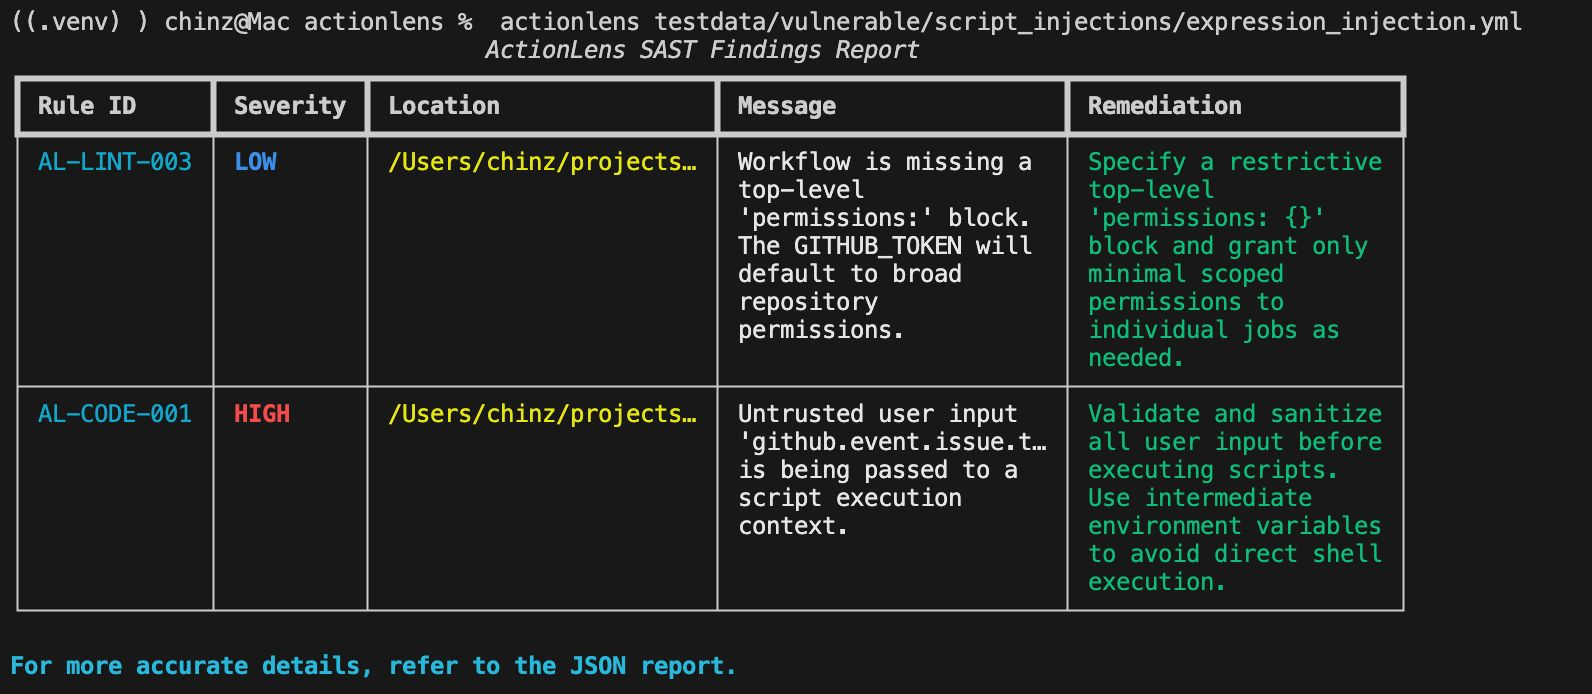
\includegraphics[width=0.95\textwidth]{bild2.jpeg}
    \caption{ActionLens output for the vulnerable script injection workflow.
    The analyzer detects the script injection through \texttt{AL-CODE-001}
    as well as a missing top-level permissions block.}
    \label{fig:script-injection-result}
\end{figure}

The second example is the vulnerable untrusted namespace workflow. In this
case, ActionLens produced five findings. The intentionally misspelled
\texttt{actons/checkout@v4} reference triggered \texttt{AL-LINT-002} with
high severity. The analyzer also detected that \texttt{setup-python} was used
under the unexpected \texttt{evil-actor} namespace. In addition, both Action
references were reported as unpinned through \texttt{AL-LINT-001}, while the
missing top-level permissions block triggered \texttt{AL-LINT-003}.

\begin{figure}[H]
    \centering
    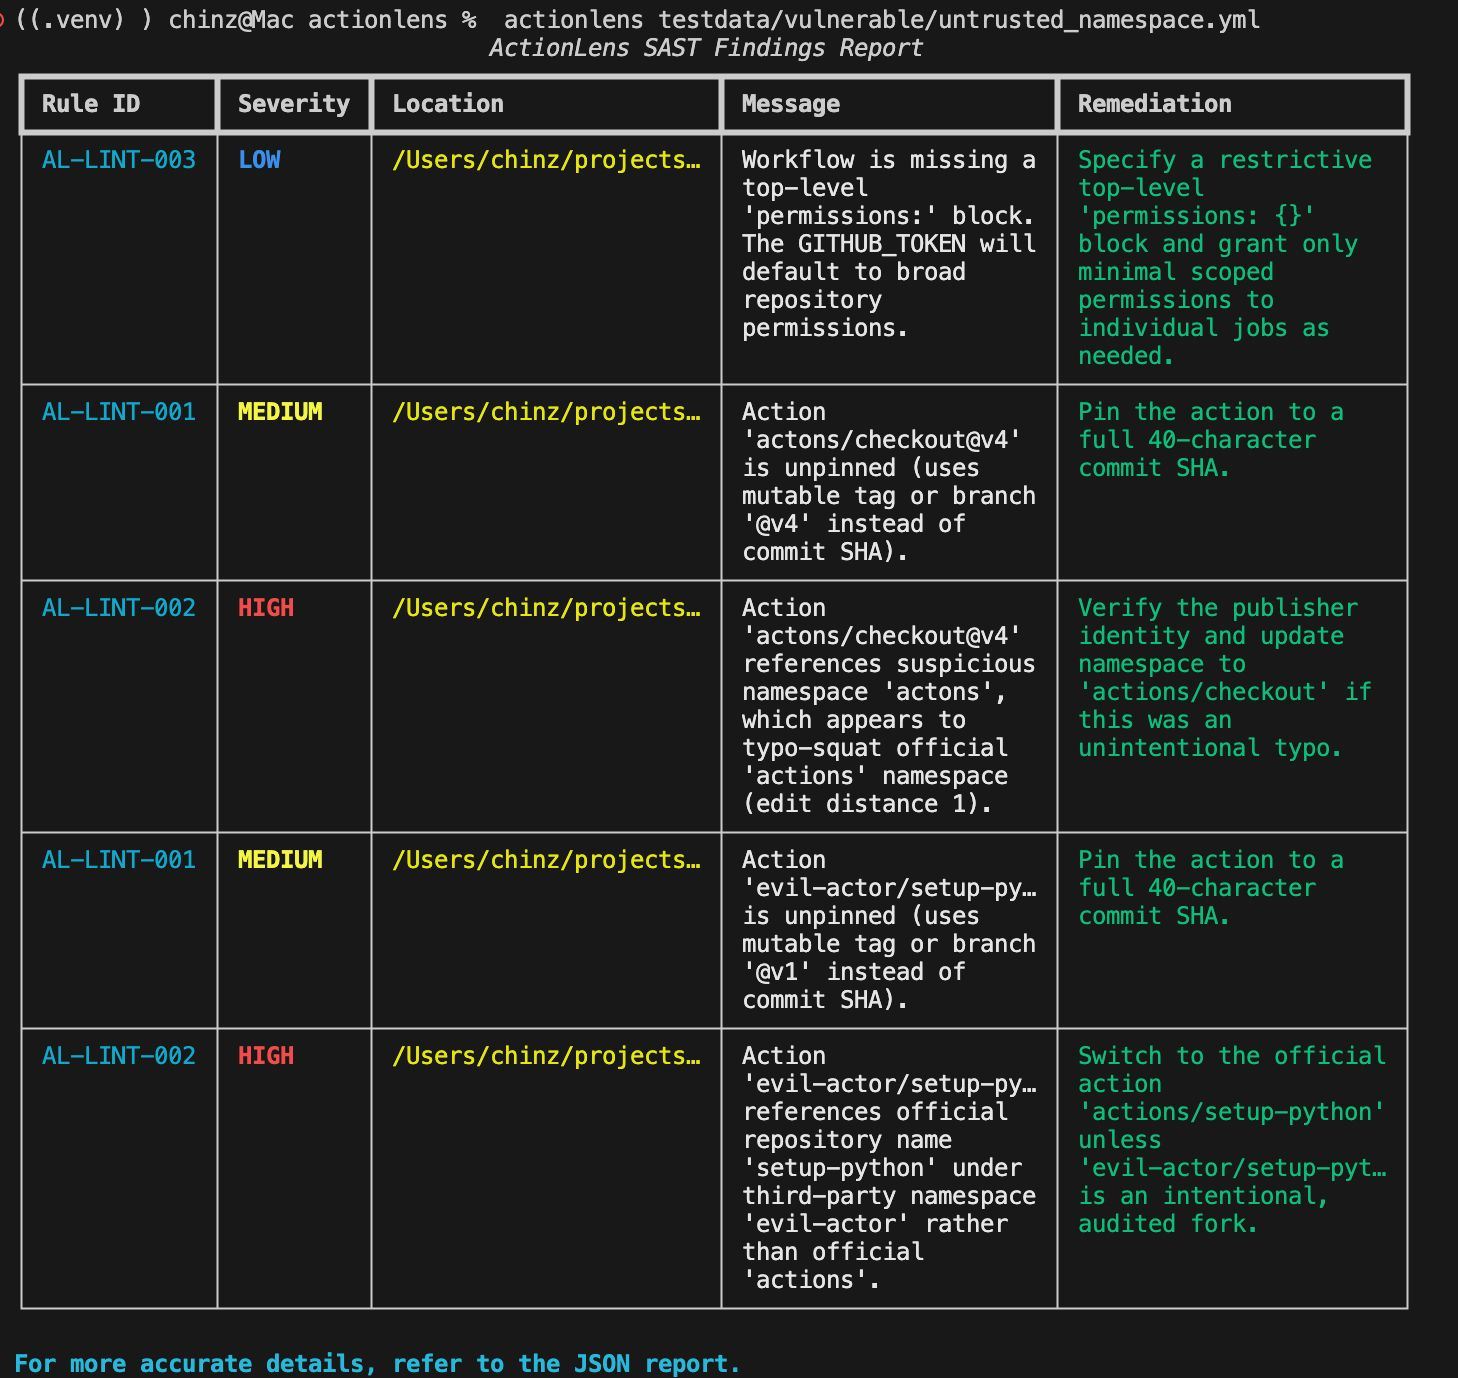
\includegraphics[width=0.95\textwidth]{bild1.jpeg}
    \caption{ActionLens output for the vulnerable untrusted namespace workflow.
    The analyzer reports findings for untrusted Action namespaces, unpinned
    Actions, and missing top-level permissions.}
    \label{fig:namespace-result}
\end{figure}

The two examples also show that the rules are evaluated independently. A
workflow created to test one specific security problem can therefore produce
additional findings when other insecure patterns are present in the same
workflow.

\clearpage
\section{Discussion}

The results show that Actionlens is able to combine different forms of static security analysis's within one and the same pipeline. Structural linting can identify configuration related vulnerabilities from the normalized AST, whilst the code-analysis rule reason about security problems regarding potential untrusted data and how it is used. This is important because not all GitHub Actions vulnerabilities can be detected by just looking for keywords or configuration values.

Our evaluation method demonstrated that the linting and code-analysis rules work independently. We saw that a workflow created to test one specific problem still could trigger findings from other rules if the file contained multiple patterns. For example, our untrusted namespace test did not only produce an \texttt{AL-LINT-002} finding, but also a unpinned Action reference and mission permissions. In a similar way, the script injection example produced both a \texttt{AL-CODE-001} finding of high severity, but also a separate permission related vulnerability. This shows that Actionlens scans the workflow for all potential security vulnerabilities rather than stop after the first possible detected problem. 

This result also affect how we recommend the output to be interpreted. The amount of findings should not be viewed as a measurement of how security dangerous the workflow is. Some finding may describe related weaknesses, and the impact from these weaknesses may depend on context such as token permissions, repository secrets, workflow trigger etc. Thus, the severity value used by Actionlens should be viewed as a warning of a risk associated with a detected pattern rather than as a assessment of real-world exploitability. 

We found it useful to utilize a normalized AST since it kept the analysis rules separate from workflow parsing. Since both the linting and code-analysis rules operate on the same internal representation, it made the architecture modular, which makes it easy to add new rules without having to implement GitHub Actions parsing again. Reusing \texttt{actionlint} also avoided the need for us to create a parser from scratch, which would have taken us too much time. On the other hand, Actionlens is now very much dependent on the information which we get from \texttt{actionlint} and the information included in the AST. 

Our taint-analysis also showed a trade-off between simplicity and semantic precision. Some vulnerabilities, such as a direct interpolation of attacker controlled GitHub context values into a \texttt{run:} command, is quite easy to identify. Other more complicated workflows may instead pass such values through several steps, therefore making it more difficult to detect the same type of vulnerability. To detect all types of cases would require a more finished data-flow model than the one we have used in our project.

We suggest that the evaluation therefore mainly should be viewed as evidence that the implemented rules behave as intended on the tested cases. Test workflows in this project were created specifically around the implemented rules and are thus considerably smaller than real-world workflows. A consequence of this is for example that our results couldn't generate any false positive/negative rates. Stronger evaluation would be possible if a larger and more real-world alike test set of workflows were used. Ideally, comparisons against existing tools such as zizmor, CodeQL or OpenSSF Scorecard would also be beneficial. 

Finally, we made a decision to exclude dynamic verification from the final project because of time constraints. Ideally though, this implementation would have helped us a lot in seeing what actually is danger or not. Actionlens can identify a potential vulnerable static pattern, but it can't confirm if this actually is exploitable during execution. The addition of dynamic verification would be very relevant for context-dependent findings such as privileged pull-request workflows. A future added layer of dynamic verification could complement Actionlens by testing certain findings in an isolated and safe environment. 

\section{Limitations and Future Work}

Due to the limited scope of the project, we chose to only focus on a small set of GitHub Actions security patterns. Thus, a workflow that produces no findings should not be viewed as secure since vulnerabilities outside the set wont be detected. The following subsections will explain most of which vulnerabilities our analyzer might miss and why. 

Our limitations of the project also affects which future work we recommend. 

\subsection{Pattern based analysis}

Several of the rules we have adapted are based on easily recognizable YAML structures/expressions. Therefore, our analyzer cannot fully determine runtime behavior such as:

\begin{verbatim}
(1)    on:
(2)        pull_request_target:
\end{verbatim}

This example together with a PR checkout might look dangerous, whilst the checked-out content could be treated only as raw data. GitHub Security Lab actually explicitly states that operations such as searching source code may be safe even if PR contents are gathered \cite{githubpwnrequests}. This could therefore flag a false positive. In the same way, a too narrowly defined set might miss the same attack if it is structured in another way. The PR contents might instead be retrieved through for example \texttt{git fetch}. This instead create false negatives, which is even more dangerous than false positives. 

Future versions of the project could therefore benefit from a broader rule coverage, such as unsafe \texttt{workflow\_run} usage, cache poisoning, dangerous credentials or insecure environment file handling \cite{githubprtarget}. We also recommend to model relationships between multiple workflow files. It would then be possible to see more vulnerabilities which only become apparent across several workflows.

\subsection{Test dataset representativeness}

The testing in this project is done within repositories and workflows which specifically are made for the project. In most real-world scenarios, this isn't the case. Thus, the evaluation environment will most likely not capture all characteristics that may happen in a real repository or workflow. 

In a similar way, the test corpus allows for accurate identification of safe/unsafe cases. But as we stated above, our manually fabricated examples are probably way simpler than the ones used in real-world workflows, which means that the results measured in the corpus should be used carefully. They can not automatically be generalized to the entire GitHub Actions system. 

If we would have had the time to test our corpus against for example zizmor, OpenSSF Scorecard, actionlint or CodeQL this would have made the evaluation substantially stronger. Alternatively, it would have been interesting to see what findings we could have gotten if we instead used SARIF like zizmor or Checkov does \cite{zizmor,checkov,githubsarif}. We therefore leave this as a recommendation for future work. 

\subsection{Commit SHA}

Our analyzer will interpret any 40-character hexadecimal string as an commit SHA. Since we don't explicitly fetch nor verify repository information, our analyzer wont be able to prove that the string actually exists, that it is the correct Action repository or if it is trustworthy \cite{githubsecurity}. 

\subsection{Severity classification}

Since the project doesn't take into account repository permissions, available secrets, branches, etc., our analyzer wont we able to label the severity of the vulnerability in a perfect way. Since severity depends on context, a solely statically assigned severity might not represent real potential impact in a particular repository. Because Actionlens only performs static analysis, it cannot confirm how a reported pattern actually might be exploited during runtime. A future dynamic verification can increase confidence in the severity findings.

Potential future work could use a larger sample of public GitHub repositories. Thus, real-world impact becomes more represented. It would also be able to measure how frequently certain patterns occur and which patterns our original analyzer missed. Additionally, using a more dynamic verification of vulnerabilities would lead to a better severity classification. Findings would then be reported separately such as for example "Static finding", "Dynamically verified finding" or "Verification inconclusive". 

\subsection{Parser and AST coverage}

Our project relies on the \texttt{actionlint} parser to correctly interpret GitHub Actions workflow syntax/expressions. It also converts the output to a smaller normalized AST for our project. Thus, the static analyzer is also limited by the information given by the parser and the normalized representation. A unsupported/incorrectly represented workflow may therefore give results might be incomplete. 

The AST does not model certain GitHub features such as strategy matrices, container, services, deployment environments, concurrency settings or additional jobs nor step properties. Security-relevant information such as these examples are therefore not visible to our analysis engine. Future work could thus extend the AST coverage whilst also improving source position tracking which would lead to more precise findings.

\section{Conclusion}

This project presented Actionlens, a static security analyzer for GitHub Actions workflows. The goal with this project was to investigate whether a combination of security linting and semantic data-flow analysis could identify a selected set of security workflow patterns. Actionlens should therefore not be seen as a general-purpose analysis framework.

Actionlens uses the existing parser from \texttt{actionlint} for GitHub Actions workflows to convert relevant information into a normalized AST. Our Python analysis engine applies six security rules that include supply-chain risks, permission and runner misconfiguration, script injections, and untrusted checkout in privileged pull-request workflows. Actionlens also support two different report outputs. The first one is a human-readable command-line table, and the other is a strucured JSON output. 

The evaluation showed that the implemented rules were able to identify security problems in the vulnerable workflow examples. Multiple independent findings could even be reported for the same workflow. This project thus demonstrates a complete static analysis pipeline from GitHub Actions parsing to security findings whilst also giving remediation advice. 

However, as stated earlier, Actionlens should not be seen as a complete security assessment. The rule coverage and the normalized AST are very limited and uses extremely simple test cases. For example, the analyzer does not verify exploitability at runtime. Future work could extend the AST and rule coverage whilst improving source-position accuracy and evaluate on real-world repositories. Other additional future work consists of adding other reporting formats such as SARIF and also introduce controlled dynamic verification for selected vulnerabilities.

Overall, the project shows a small but modular analyzer which combines structural linting with semantic analysis to detect several security issues in GitHub Actions workflows. It also produces findings that are understandable for the user in two different formats. 

\section{Individual Contributions}

We decided to split the project in groups of two. Alexander and Elsa focused on Dataflow and Taint Analysis, whilst Chinmay and Tilda instead researched Security Linters and integration. For each of these two groups, one member was chosen as a coder (Alexander and Chinmay), whilst the other member focused on report writing (Elsa and Tilda). 

\subsection{Alexander Götting}
My main contribution to the project was the logic behind Actionlens’s taint analysis. This began with extensive research into what taint analysis is and how it applies to code analysis. Since the team agreed not to build our own abstract syntax tree, I tested several existing options and we settled on the one provided by Go’s Actionlint, which balances a rich feature set with the readability of Go.

Because the group preferred working in Python, I implemented the taint graph logic in Python. The taint graph is essentially a simple wrapper around NetworkX graphs. The hardest part, and core of my work, was defining robust rules for adding edges, since a GitHub workflow offers many valid constructs that can lead to code execution, and the algorithm must recognize many different kinds of sinks. Once the graph is built, finding potentially tainted paths reduces to calling NetworkX’s standard path-finding APIs. Finally, I integrated my logic into the interfaces and orchestrator developed by Chinmay and wrote meaningful tests.

I authored two rules, script\_injection.py and untrusted\_checkout.py, which are the only ones that need taint graph logic to avoid false positives. They trace the path an untrusted input takes, including when it is written to Github\_Output and later read back. Additionally, my tests provide the ability to generate a visual HTML of the produced taint graphs for debugging or educational purposes. 

\subsection{Chinmay Prawah Pant}
My main contribution to the project has been the overall design, planning and the core implementation of ActionLens. At the start of the project, I brainstormed several project ideas with the group, looking at both their real-world value and how well they matched the skills in our team. I proposed static analysis of GitHub Actions workflows and the group agreed. I defined the scope of the tool, set up the repository, and decided on the architecture. We chose to write the parser in Go so that we could reuse actionlint, an existing actions workflow parser, and detection engine is written in Python.

I built the complete parser as a wrapper around actionlint. It reads a workflow file and converts actionlint’s syntax tree into a simpler JSON format that the Python engine reads. It also holds every embedded expression, such as references to issue titles or branch names, together with where in the step it appears. I also wrote the Go tests for the parser and the Python models that validate its output.

On the Python side, I created the SAST orchestrator, which loads a workflow, runs every registered rule on it, and collects the findings. I designed the rule interface and a single rule catalog that stores each rule’s severity, description, CWE, OWASP CI/CD category and remediation advice. This made it easy to add or change rules as the research evolved. I implemented four lint rules, with their test workflows and tests. They cover unpinned actions, untrusted or typo-squatted action namespaces, missing or over-scoped permissions, and self-hosted runners. I also designed and developed the reporting formatter and the command-line interface, which show the findings as a table in the terminal or as JSON.

I researched and defined the six vulnerabilities that ActionLens detects and decided the scope of each one. For the two data-flow vulnerabilities, this built on Elsa’s research into script injection and the Argus approach. I documented all six in the vulnerability matrix, where each one has an exploit scenario and is mapped to a CWE and an OWASP CI/CD risk. I also wrote the architecture and development documentation, the README, and the research notes on taint sources, propagators and sinks.

I worked with Alexander on the data-flow and taint-analysis part, and he implemented the taint rules. We discussed how the taint graph should work and what we could realistically cover within the time frame of the project. I later extended the lists of untrusted contexts and execution sinks used by the script-injection rule, and wrote more complex test workflows for it.

Finally, I coordinated with Elsa and Tilda on the direction and progress of the project. I also cross-checked the report against the implementation to make sure it described what ActionLens actually does.

\subsection{Elsa Kieffer}

My main contribution to the project has been report writing and research related
to the data-flow and taint-analysis part of ActionLens. I worked together with
Alexander on this part of the project, where he focused mainly on the
implementation while I focused on understanding the security problems, finding
relevant research, and documenting how our approach works.

Early in the project, I researched script injection vulnerabilities in GitHub
Actions and looked at examples of how attacker-controlled values, such as issue
titles, pull-request data, comments, and branch names, can reach shell commands.
I also studied Argus and its source-to-sink approach to taint analysis. This
research was used when deciding how we could simplify data-flow analysis to fit
the scope and time frame of our project.

A large part of my work has also been writing and structuring the report
together with Tilda. I worked especially on the threat model, design and
implementation, evaluation method, and results. For these sections, I went
through the implementation and test cases together with the developers to make
sure that the report described what ActionLens actually implements. 

\subsection{Tilda L. Aderud}

My main contribution to this project has been focused on report writing and research regarding security-focused linting. Early on in the project, I investigated how linting may be applied to GitHub Actions workflows and what security problems could be detected via analyzing workflow files. I mostly studied unpinned third-party Actions and unsafe usage of \texttt{pull\_request\_target}. Together with Chinmay, I gathered information about how these problems arise, what they look like, and what our analyzer should be looking out for. 

Further, I also contributed to defining the scope of the linting component together with Chinmay. We decided how different findings should be structured, as well as how vulnerable/secure test cases were to be organized. Additionally, we suggested that the evaluation of false positives/negatives later could be evaluated using a controlled workflow corpus. Unfortunately due to time constraints, we did not have enough resources to implement this. 

The most substantial part of my work has been put into writing the report. Together with Elsa, we have written the entire report with some help during the results part from Alexander and Chinmay. For the report writing, a lot of research also went into gathering information about similar work, such as \textsc{Argus}, CodeQL, zizmor, OpenSSF Scorecard, Checkov and actionlint. The research on these related tools gave me insight in how our project eventually could evolve. Large portions of the external sources found in the report were made by me, whilst Elsa took care of formatting and inserting the citations at the correct places. 

Lastly, I helped with identifying limitations to our approach, such as severity classification and our dependency on \texttt{actionlint}. 

\bibliographystyle{IEEEtran}
\bibliography{references}

\end{document}
